\section{Project Description}
The research described here proposes a new technique for verification of task parallel programs with the help of computation graphs. It uses Habanero Java as an exemplar of task parallel languages. Habanero Java language is a task parallel programming language built as an extension to X10 language. It includes a set of powerful parallel programming constructs that can be used to create programs that are inherently safe. HJ programs can be run on any JVM including Java 8 JVM.  The Habanero Java language puts particular emphasis on the usability and safety of parallel programming constructs. For Example, no HJ program written using async, finish, isolated and phaser constructs can create a logical deadlock cycle.

\subsection{HJ constructs}
Habanero Java consists of a wide range of constructs for parallel programming.
\begin{enumerate}
\item \textbf{Task Spawn and Join} - Async and finish constructs are used to create and join tasks created by a parent process. The statement async(() $ \rightarrow \langle$stmt$\rangle$) creates a new task that can logically execute in parallel with its parent task. The Finish method is used to represent join in Habanero Java. The task executing finish(() $ \rightarrow \langle$stmt$\rangle$) has to wait for all the tasks running inside stmt to finish before it can move on.
\item \textbf{Loop Parallelism} - The forall and foreach constructs in HJ are used for loop parallelism. An implicit finish is included at the end of forall iterations whereas foreach iterations do not have an implicit finish. 
\item \textbf{Coordination Constructs} - There are often dependencies among parallel tasks. To coordinate the execution of the parallel tasks, Habanero Java provides some constructs such as isolated, futures, data-driven futures and phasers.
\begin{enumerate}
\item \textbf{Isolated}
Most of the concurrently running processes have the need to synchronize the access to the shared variables. The isolated statements allow only one process at a time to access referenced shared variables. Isolated statements create performance bottlenecks in moderate to high contention systems. HJ also provides object-based isolation which provides better performance.
\item \textbf{Futures} - HJ supports returning values from a newly created child task to the parent task with the help of futures. The statement HjFuture$\langle$T$\rangle$ f = future $\langle$T$\rangle$ (() $ \rightarrow \langle$expr$\rangle$) creates a new child task which executes expr and the result of this execution can be obtained by the parent task by calling f.get() method.
\item \textbf{Data-driven futures} - DDFs are an extension to futures. Any async can register on a DDF as a consumer causing the execution of the async to be delayed until a value becomes available in the DDF. The exact syntax for an async waiting on a DDF is as follows: asyncAwait(ddf1, ... , ddfN, () $\rightarrow$ stmt). An async waiting on a chain of DDFs can only begin executing after a put() has been invoked on all the DDFs.
\item \textbf{Phasers} - Phasers help in point-to-point synchronization. Each task has the option of registering with a phaser in signal-only/wait-only mode for producer/consumer synchronization or signal-wait mode for barrier synchronization. A task may be registered on multiple phasers, and a phaser may have multiple tasks registered on it. Phasers ensure deadlock freedom when programmers use only the next statements in their programs. In programs where tasks are involved with multiple point-to-point coordination, explicit use of doWait() and doSignal() on multiple phasers might be required.  
\end{enumerate}
\end{enumerate}

\subsection{Computation Graphs}
The execution of an task parallel program can be represented in the form of a computation graph. A computation graph of a program is a directed acyclic graph(DAG) structure that represents the sequence of execution of tasks in the parallel program. A computation graph can be represented as G = $\langle$V, E$\rangle$ where
\begin{itemize}
\item V represents a set of nodes such that  each node represents a step consisting of an arbitrary sequential computation and
\item E represents a set of directed edges that represent ordering constraints. The various types of edges in a computation graph are:
\begin{enumerate}
 \item \textbf{Spawn edges} - They connect steps in parent tasks to steps in child async tasks. When an async is created, a spawn edge is inserted between the step that ends with the async in the parent task and the step that starts the async body in the new child task.
\item \textbf{Join edges} - They connect steps in descendant tasks to steps in the tasks containing their Immediately Enclosing Finish (IEF) instances. When an async terminates, a join edge is inserted from the last step in the async to the step that follows the IEF operation in the task containing the IEF operation.
\item \textbf{Continue edges} - They capture sequencing of steps within a task - all steps within the same task are connected by a chain of continue edges.
 \end{enumerate} 
\end{itemize}

\subsection{HJ example with its computation graph representation}
Fig.1 shows an example program written in Habanero Java. In this example, the main process starts two new processes running in parallel with the process. The main process has to stop its execution at the end of finish block and wait for the child processes to complete their execution before the main process can proceed further. This results in a computation graph shown in fig. 2. 

\begin{figure}[h!]
  \caption{Example HJ Program}
    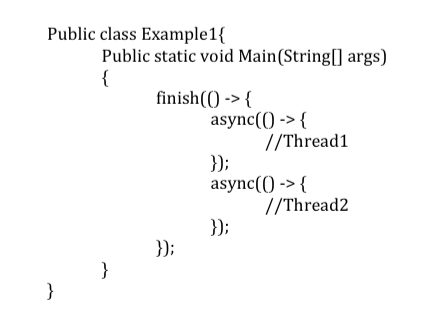
\includegraphics[scale=0.5]{../figs/Fig1.jpg} 
\end{figure}
\begin{figure}[h!]
  \caption{Example HJ Program}
    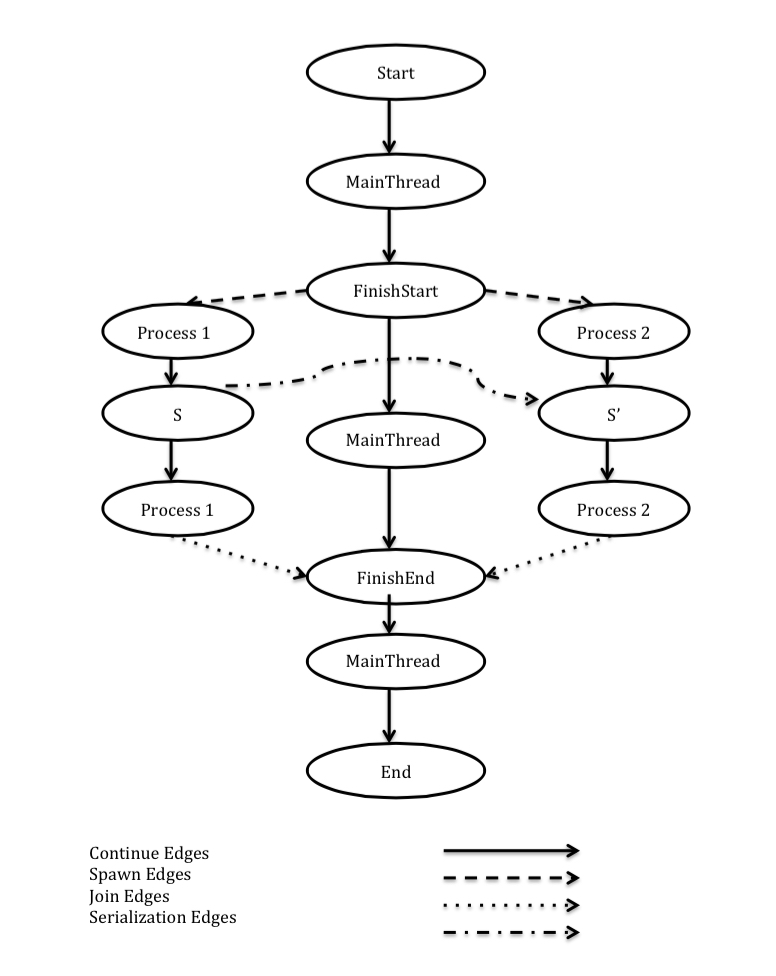
\includegraphics[scale=0.5]{../figs/Fig2.jpg}
\end{figure}
\subsection{Verification of Properties of Task Parallel Programs}
The following properties of task parallel programs can be verified using computation graphs.
\subsubsection{Data Race}
Data races occur in parallel programs when two or more tasks try to access shared variables such that at least one of the accesses is a 'write'. Data races cause the output of the program to become non-deterministic. Data races can be detected in a computation graph when two parallel nodes in the graph access a memory location and atleast one of the operations tries to modify it. A Topological traversal of the graph gives the order of execution of the various tasks. All the nodes that occur between  a pair of Finish-start and Finish-end nodes execute in parallel. The global memory accesses by these processes have to be checked and if conflicting memory-accesses are observed, then a data race should be reported.
\subsubsection{Determinism}
Determinism refers to obtaining the same result from a parallel program for a given input. There are different definitions that determine the degree of determinism in parallel programs.
\begin{enumerate}
\item
\textbf{Internal (or structural) determinism:\\}
This type of determinism requires the parallel program to not only produce the same output for a given input, but also to produce a unique computation graph for a given input. A program is internally deterministic only if it is free of data-races.
\item
\textbf{External (or functional) determinism:\\}
External determinism requires the parallel program to produce the same output when run on the same input. Program's executions for a given input may be different, but they ultimately produce the same output. When a program is data-race free, it is externally deterministic as well. In the presence of data-races, a program is externally deterministic if every pair of concurrent operators commute.3
\end{enumerate}
\subsubsection{Deadlock}
A Deadlock arises in parallel programs when two or more processes are waiting to acquire resources held by other processes without making any progress. The necessary conditions (known as the Coffman conditions) for a deadlock to arise are as follows:
\begin{enumerate}
\item 
{Mutual Exclusion:} At least one resource must be held in a non share-able mode. Only one process can access the resource at any given time. 
\item
{Hold and Wait:} This condition refers to a process holding a non share-able resource and trying to acquire another one.
\item
{No Preemption}
If no tasks are allowed to preempt other tasks from holding the locks for certain resources, it can cause a deadlock to happen.
\item
{Circular Wait} Circular wait implies that there are at least two tasks that are waiting on resources held by the other tasks.
\end{enumerate}
If all the computation graph structures created for all possible inputs of a program do not encounter any processes getting blocked during execution, then we can say the program is deadlock-free.
